\documentclass[]{article}
\usepackage{lmodern}
\usepackage[compact]{titlesec}
\usepackage{amssymb,amsmath}
\usepackage{ifxetex,ifluatex}
\usepackage{fixltx2e} % provides \textsubscript
\ifnum 0\ifxetex 1\fi\ifluatex 1\fi=0 % if pdftex
  \usepackage[T1]{fontenc}
  \usepackage[utf8]{inputenc}
\else % if luatex or xelatex
  \ifxetex
    \usepackage{mathspec}
  \else
    \usepackage{fontspec}
  \fi
  \defaultfontfeatures{Ligatures=TeX,Scale=MatchLowercase}
\fi
% use upquote if available, for straight quotes in verbatim environments
\IfFileExists{upquote.sty}{\usepackage{upquote}}{}
% use microtype if available
\IfFileExists{microtype.sty}{%
\usepackage{microtype}
\UseMicrotypeSet[protrusion]{basicmath} % disable protrusion for tt fonts
}{}
\usepackage[margin=1in]{geometry}
\usepackage{hyperref}
\hypersetup{unicode=true,
            pdftitle={Visualizing Text},
            pdfauthor={Darryl Buswell},
            pdfborder={0 0 0},
            breaklinks=true}
\urlstyle{same}  % don't use monospace font for urls
\usepackage{longtable,booktabs}
\usepackage{graphicx,grffile}
\makeatletter
\def\maxwidth{\ifdim\Gin@nat@width>\linewidth\linewidth\else\Gin@nat@width\fi}
\def\maxheight{\ifdim\Gin@nat@height>\textheight\textheight\else\Gin@nat@height\fi}
\makeatother
% Scale images if necessary, so that they will not overflow the page
% margins by default, and it is still possible to overwrite the defaults
% using explicit options in \includegraphics[width, height, ...]{}
\setkeys{Gin}{width=\maxwidth,height=\maxheight,keepaspectratio}
\IfFileExists{parskip.sty}{%
\usepackage{parskip}
}{% else
\setlength{\parindent}{0pt}
\setlength{\parskip}{6pt plus 2pt minus 1pt}
}
\setlength{\emergencystretch}{3em}  % prevent overfull lines
\providecommand{\tightlist}{%
  \setlength{\itemsep}{0pt}\setlength{\parskip}{0pt}}
\setcounter{secnumdepth}{0}
% Redefines (sub)paragraphs to behave more like sections
\ifx\paragraph\undefined\else
\let\oldparagraph\paragraph
\renewcommand{\paragraph}[1]{\oldparagraph{#1}\mbox{}}
\fi
\ifx\subparagraph\undefined\else
\let\oldsubparagraph\subparagraph
\renewcommand{\subparagraph}[1]{\oldsubparagraph{#1}\mbox{}}
\fi

%%% Use protect on footnotes to avoid problems with footnotes in titles
\let\rmarkdownfootnote\footnote%
\def\footnote{\protect\rmarkdownfootnote}

%%% Change title format to be more compact
\usepackage{titling}

% Create subtitle command for use in maketitle
\newcommand{\subtitle}[1]{
  \posttitle{
    \begin{center}\large#1\end{center}
    }
}

\setlength{\droptitle}{-2em}
  \title{Visualizing Text}
  \pretitle{\vspace{\droptitle}\centering\huge}
  \posttitle{\par}
\subtitle{MSPA PREDICT 455-DL-SEC55}
  \author{Darryl Buswell}
  \preauthor{\centering\large\emph}
  \postauthor{\par}
  \date{}
  \predate{}\postdate{}

\begin{document}
\maketitle

\newpage

\section{1 Introduction}\label{introduction}

This assignment explores text from Abraham Lincoln's four Addresses
(Addresses), with the aim to identify and compare trends in each Address
using visualization techniques. Full text for each speech is available
from the GitHub repository, Web and Network Data Science (WNDS 2016).
Table A1 shows a summary of properties for each of the four files used.
Each file is in text format, and each represents an Address made by
Abraham Lincoln over the years 1861, 1862, 1863 and 1864.

\section{2 Data Pre-Processing}\label{data-pre-processing}

Data was pre-processed to remove punctuation, digits, stop words and
excess white space between words. This transformation resulted in
retention of words with meaning which can be aggregated and analyzed.
The package `tm' was leveraged to carry out transformations and to
convert the text into a `corpus'. A separate corpus was created for each
of the original datasets and for an aggregated dataset which contains
text from all four or the original datasets. Table A2 summarizes each of
the applied transformations, as well as the order in which they were
applied.

A Term Document Matrix (TDM) was created for each corpus, which consists
of a matrix of word documents against the frequency by which they
appear. A separate TDM was created for single N-gram's (e.g. `United'),
two joining N-grams (e.g. `United States'), and three joining N-grams
(e.g. `United States America'). Tokenizing over N-gram sequences
facilitated the exploration of not only Lincoln's use of single words,
but also the use of two and three word combinations.

Table A3 shows the number of unique N-gram occurrences within each TDM.
Note that the number of unique unigrams which occur over all four
Addresses is much less than the sum of unique unigrams which occur over
each. This suggests that many unigram occurrences were repeated over
each Address.

\section{3 Data Exploration}\label{data-exploration}

Frequently appearing N-grams over all four (combined) Addresses are
represented as word clouds and bar plots in Figures B1 to B6. Figure B1
and B2 show that the most common unigrams over all four Addresses were
`the', `congress', and `states', which occured 43, 29, and 28 times,
respectively. The most common bigram over all four Addresses was `united
states', followed by `i recommend' and `circuit courts'. The amount of
occurrences of `united states' comes in at 9, greatly outweighing `i
recommend' and `circuit courts' which showed 5 and 4 occurrences,
respectively. The most common trigrams were `circuit judges provided'
and `confiscate property used'.

Figure B7 presents a comparison word cloud which shows the year of each
Address in a 2x2 grid. The unigrams occured at a high frequency across
all Addresses, but occurred most frequently in the year specified in the
word cloud. Some results were suprising, for example, the Battle of Fort
Sumter occurred over 1861, however the highest use of the unigram
`naval' occurred during the 1863 Address. Also, the American Civil War
started in 1861, yet the unigram `war' was mentioned most often in 1864.

We can relax the focus on bigrams and trigrams within each Address, and
instead draw attention to correlations between each unigram. For this,
we can leverage the `biocLite' package. A visual representation of
unigram correlations over all four (combined) Addresses is shown in
Figure B8. A correlation threshold of 0.2 was applied to the unigram
correlations and a limit was set for the number of unigrams shown. Not
surprisingly, unigrams previously reported to have high frequencies are
shown to have high correlations.

Finally, we can use the R package `topicmodels' to implement a Latent
Dirichlet Allocation (LDA) model. The LDA can be used to classify themes
within each Address. For the most part, default parameter options were
used for the LDA implementation, however both the number of topics and
the number of unigrams within each topic was set at four and ten
respectively. The list of topics and included unigrams is shown in Table
A4. It is difficult to define any of the topics based on their included
unigrams, and results could not be improved by modifying either the
topic count or number of included unigrams. However, applying this
routine to a larger text corpus may improve the results.

A bar plot was then used to represent how often the unigrams within each
topic were referred to for each Address. Note that the proportion of use
of each unigram (proportion of topic reference) was calculated by
ignoring the frequency of any unigrams which are not within one of the
four topics. As Figure B9 shows, the proportion of topic reference does
not change radically between each Address. Do note that there was a
slight increase in occurrences of unigrams within Topic 3 between the
1861 and 1862 Address, which coincided with a decrease in occurrences of
unigrams within Topic 2. There was also a slight increase in occurrences
of unigrams within Topic 1 between 1862 and 1863, which coincided with a
decrease in occurrences of unigrams within Topic 4.

\section{4 Conclusion}\label{conclusion}

We were able to process the dataset in order to find common unigram,
bigram, and trigram frequencies, find correlations between unigrams and
classify the text into topics. The powerful visualization packages
within R also allowed these text transformations to be presented using a
combination of wordclouds, comparison clouds, barplots, stacked barplots
and correlation diagrams. For future work, it may be worth applying the
same process to a larger corpus of text, potentially capturing all
Addresses made over a number of administrations. Doing so may expose new
trends within the underlying data and allow a wider set of inferences to
be made.

\newpage

\section{Appendix A Table Output}\label{appendix-a-table-output}

\subsection{Table A1 Dataset Summary}\label{table-a1-dataset-summary}

\begin{longtable}[]{@{}llll@{}}
\toprule
File (name) & Size (mb) & Lines (no.) & Longest Line
(chars)\tabularnewline
\midrule
\endhead
R\_W\_Lincoln\_1861.txt & 0.04 & 161 & 1887\tabularnewline
R\_W\_Lincoln\_1862.txt & 0.05 & 215 & 3149\tabularnewline
R\_W\_Lincoln\_1863.txt & 0.04 & 113 & 2810\tabularnewline
R\_W\_Lincoln\_1864.txt & 0.03 & 167 & 2376\tabularnewline
\bottomrule
\end{longtable}

\subsection{Table A2 Pre-processing
Routine}\label{table-a2-pre-processing-routine}

\begin{longtable}[]{@{}ll@{}}
\toprule
Order & Transformation\tabularnewline
\midrule
\endhead
1 & Convert from UTF-8 to ASCII\tabularnewline
2 & Remove punctuation\tabularnewline
3 & Remove digits\tabularnewline
4 & Remove English stopwords (e.g.~to, a, is)\tabularnewline
5 & Convert text to lowercase\tabularnewline
6 & Strip all whitespace\tabularnewline
\bottomrule
\end{longtable}

\subsection{Table A3 N-gram Audit}\label{table-a3-n-gram-audit}

\begin{longtable}[]{@{}llll@{}}
\toprule
Union Address & Unigram & Bigram & Trigram\tabularnewline
\midrule
\endhead
Lincoln 1861 & 1651 & 3308 & 3369\tabularnewline
Lincoln 1862 & 1782 & 3987 & 4103\tabularnewline
Lincoln 1863 & 1511 & 2966 & 3047\tabularnewline
Lincoln 1864 & 1480 & 2823 & 2889\tabularnewline
Lincoln 1861-1864 & 3686 & 12372 & 13238\tabularnewline
\bottomrule
\end{longtable}

\subsection{Table A4 Topic Terms}\label{table-a4-topic-terms}

\begin{longtable}[]{@{}llll@{}}
\toprule
Topic 1 & Topic 2 & Topic 3 & Topic 4\tabularnewline
\midrule
\endhead
the & the & the & the\tabularnewline
will & states & states & will\tabularnewline
congress & year & will & states\tabularnewline
can & united & labor & can\tabularnewline
government & department & people & national\tabularnewline
upon & receipts & time & war\tabularnewline
country & upon & union & now\tabularnewline
general & great & congress & may\tabularnewline
states & treasury & shall & new\tabularnewline
may & last & upon & great\tabularnewline
\bottomrule
\end{longtable}

\newpage

\section{Appendix B Figure Output}\label{appendix-b-figure-output}

\subsection{Figure B1 Lincoln SoUA 1861-1864 Unigram
Wordcloud}\label{figure-b1-lincoln-soua-1861-1864-unigram-wordcloud}

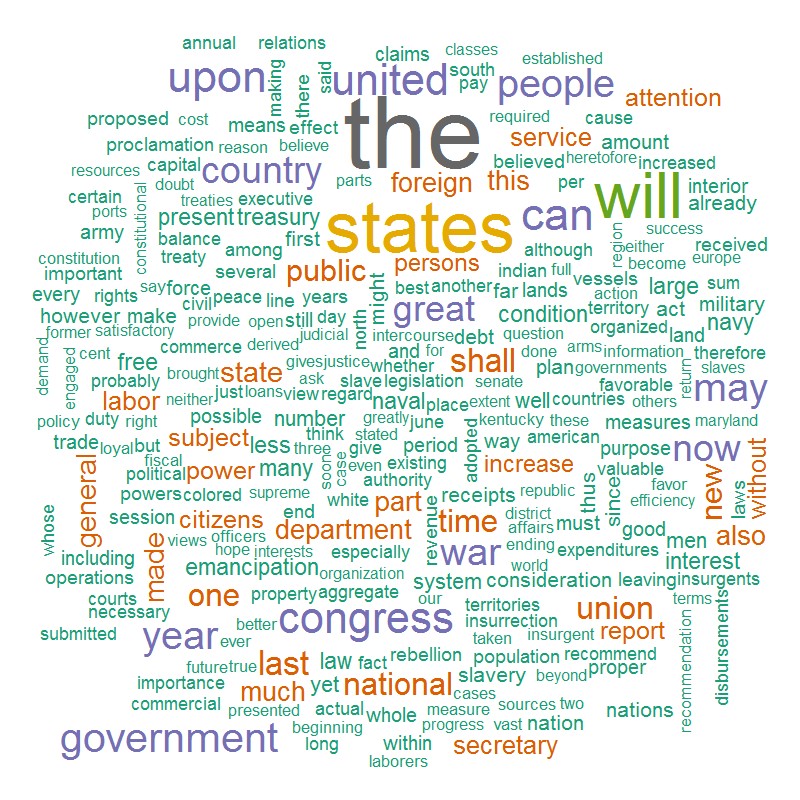
\includegraphics[height=8.33333in]{images/Lincolndata_unigram_wc.png}

\subsection{Figure B2 Lincoln SoUA 1861-1864 Unigram (Frequency
\textgreater{}=60)}\label{figure-b2-lincoln-soua-1861-1864-unigram-frequency-60}

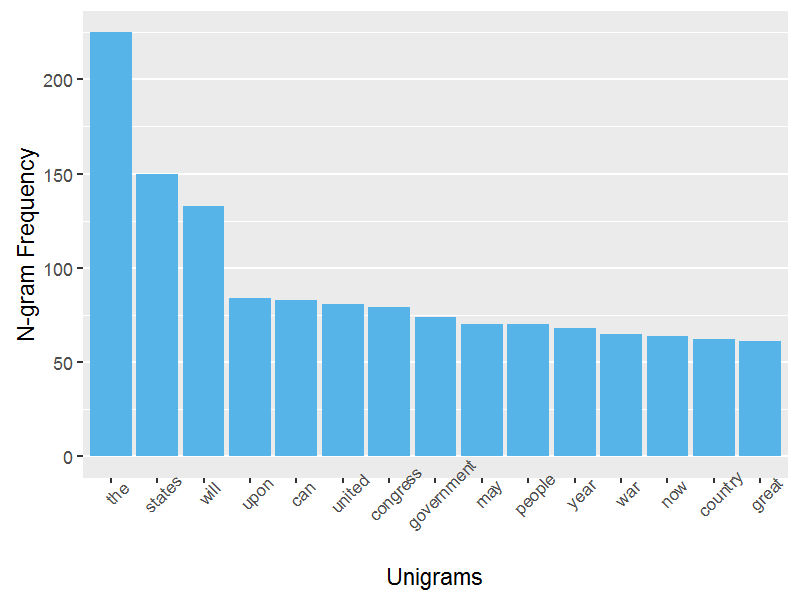
\includegraphics[height=8.33333in]{images/Lincolndata_unigram_bar.png}

\newpage

\subsection{Figure B3 Lincoln SoUA 1861-1864 Bigram
Wordcloud}\label{figure-b3-lincoln-soua-1861-1864-bigram-wordcloud}

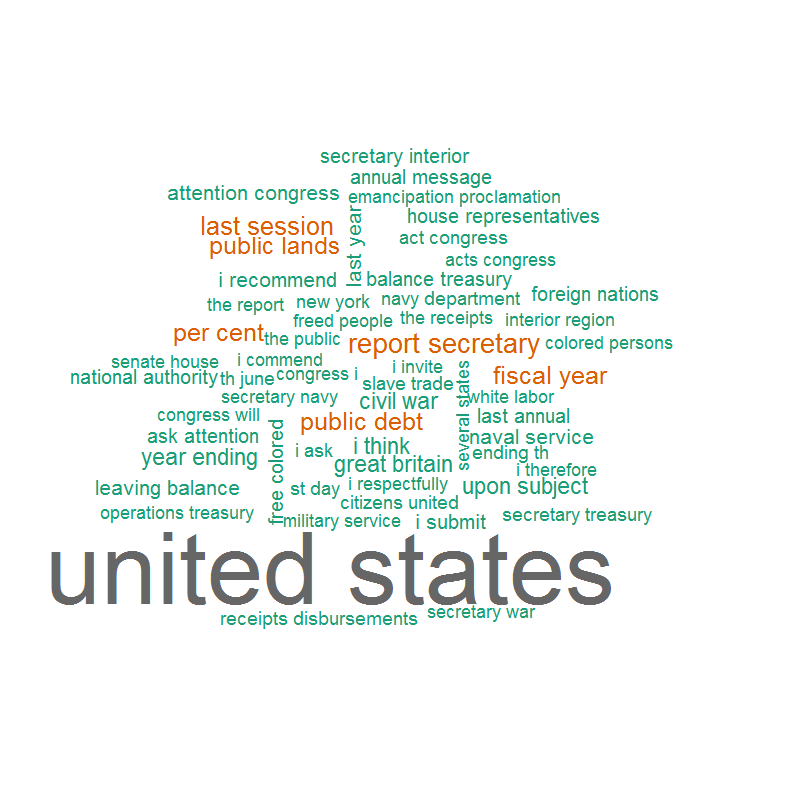
\includegraphics[height=8.33333in]{images/Lincolndata_bigram_wc.png}

\vfill

\subsection{Figure B4 Lincoln SoUA 1861-1864 Bigram (Frequency
\textgreater{}=9)}\label{figure-b4-lincoln-soua-1861-1864-bigram-frequency-9}

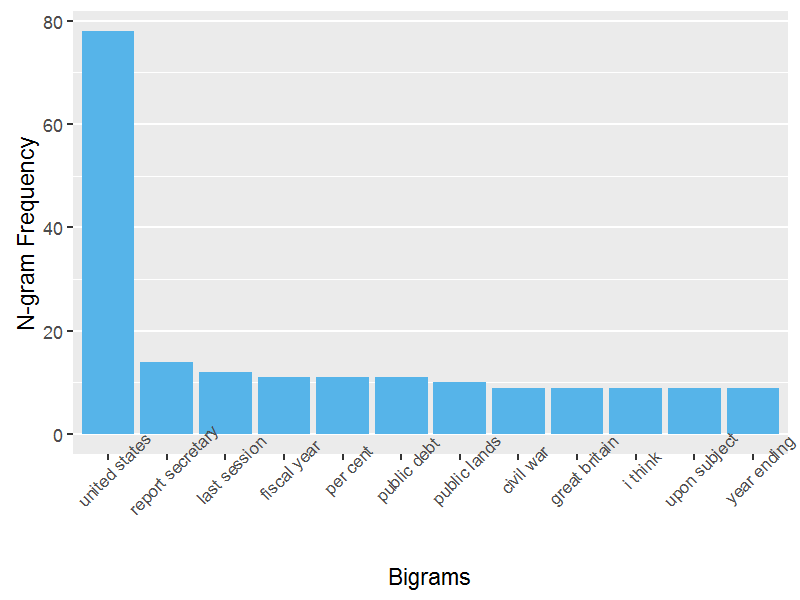
\includegraphics[height=8.33333in]{images/Lincolndata_bigram_bar.png}

\newpage

\subsection{Figure B5 Lincoln SoUA 1861-1864 Trigram
Wordcloud}\label{figure-b5-lincoln-soua-1861-1864-trigram-wordcloud}

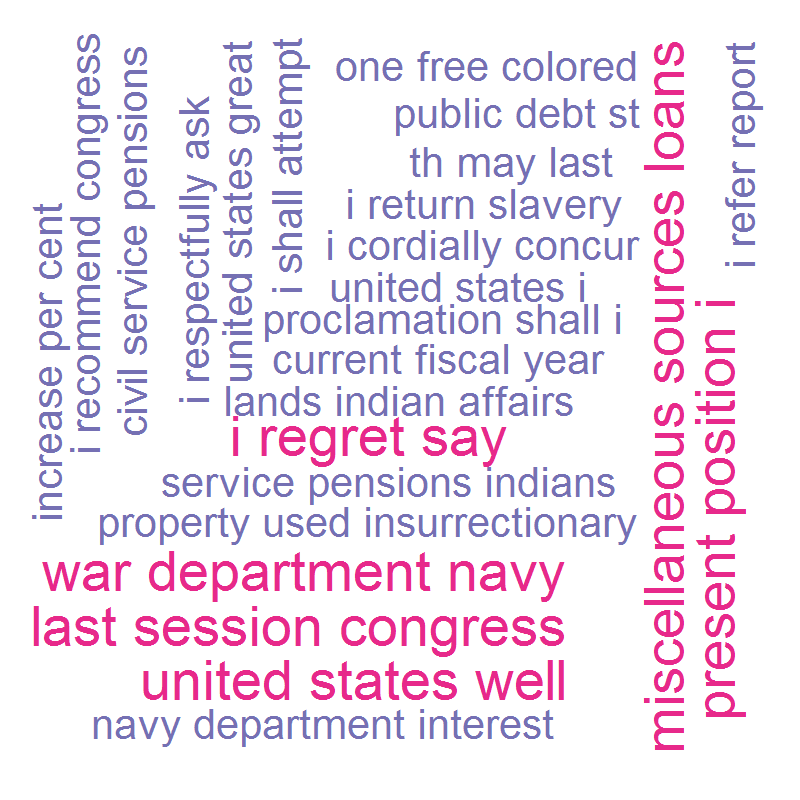
\includegraphics[height=8.33333in]{images/Lincolndata_trigram_wc.png}

\vfill

\subsection{Figure B6 Lincoln SoUA 1861-1864 Trigram (Frequency
\textgreater{}=4)}\label{figure-b6-lincoln-soua-1861-1864-trigram-frequency-4}

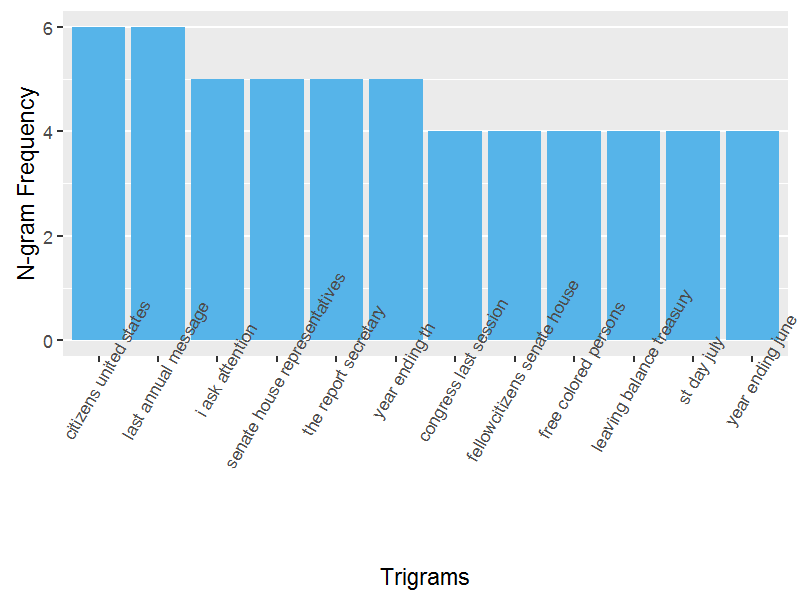
\includegraphics[height=8.33333in]{images/Lincolndata_trigram_bar.png}

\subsection{Figure B7 Lincoln SoUA 1861-1864 Unigram Comparison
Cloud}\label{figure-b7-lincoln-soua-1861-1864-unigram-comparison-cloud}

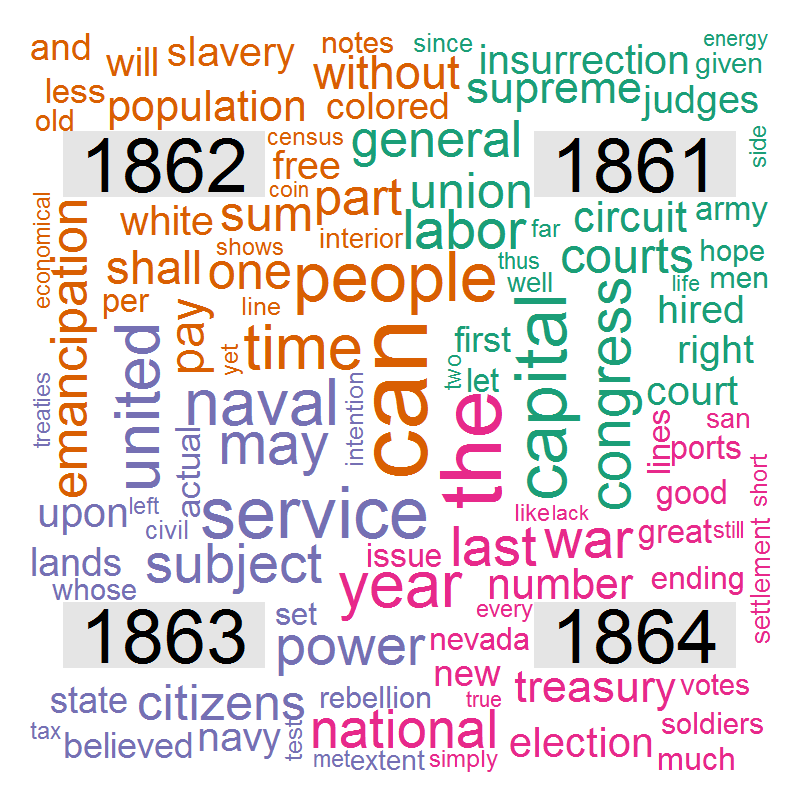
\includegraphics[height=7.29167in]{images/Lincolndata_compcloud.png}

\subsection{Figure B8 Lincoln SoUA 1861-1864 Correlation
Cloud}\label{figure-b8-lincoln-soua-1861-1864-correlation-cloud}

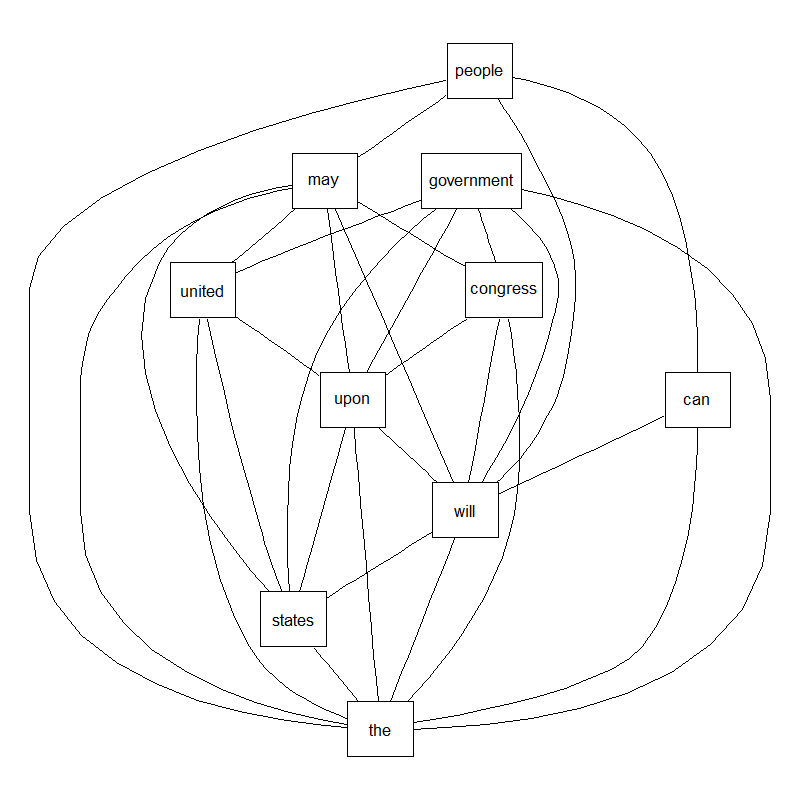
\includegraphics[height=7.29167in]{images/Lincolndata_corrcloud.png}

\subsection{Figure B9 Lincoln SoUA 1861-1864 Topic
References}\label{figure-b9-lincoln-soua-1861-1864-topic-references}

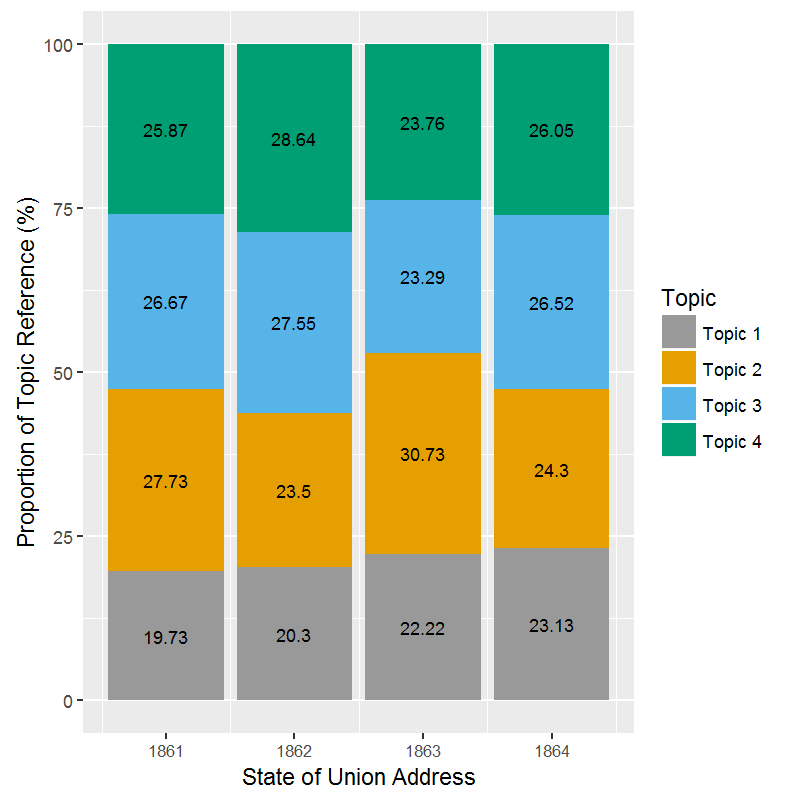
\includegraphics[width=8.33333in,height=4.16667in]{images/Lincolndata_topictrend.png}

\newpage

\section*{References}\label{references}
\addcontentsline{toc}{section}{References}

\hypertarget{refs}{}
\hypertarget{ref-github:wnds}{}
WNDS. 2016. ``GitHub: Web and Network Data Science.''
\url{https://github.com/mtpa/wnds}.


\end{document}
